% ICRA paper skeleton for tactile-forecasting.
% Format: IEEE RAS/PaperCept conference template (ieeeconf, US Letter, 10 pt).
% Before submission:
%   1) replace the anonymous author block after the review phase;
%   2) replace the four boxed figure placeholders with final vector figures;
%   3) regenerate every table directly from the frozen result CSVs;
%   4) remove all TODO comments and confirm the current ICRA page-limit policy.
% Important scientific guardrails:
%   - class-specific R^2 and Delta R^2 are primary for the smooth/abrupt test;
%   - skill vs. persistence is diagnostic and its aggregation must be declared;
%   - do not mix clip-balanced and frame-pooled numbers in one comparison.

\documentclass[letterpaper, 10 pt, conference]{ieeeconf}

\IEEEoverridecommandlockouts
\overrideIEEEmargins

\usepackage{cite}
\usepackage{amsmath,amssymb,amsfonts}
\usepackage{booktabs}
\usepackage{graphicx}
\usepackage{textcomp}
\usepackage{xcolor}
\usepackage{url}
\usepackage[hidelinks]{hyperref}
\graphicspath{{figures/}}

\newcommand{\Rdiff}{\mathcal{R}}
\newcommand{\Rtwo}{R^{2}}
\newcommand{\dRtwo}{\Delta R^{2}}
\newcommand{\model}[1]{\textsc{#1}}
\newcommand{\placeholderfigure}[2]{%
  \fbox{\parbox[c][#1][c]{0.95\linewidth}{\centering\footnotesize #2}}}

\begin{document}

\title{\LARGE \bf
When Is Touch Predictable? Temporal Structure and the Limits of One-Second Tactile Forecasting
}

% Keep the submission anonymous if required by the current ICRA call for papers.
% Replace this block with the official author/affiliation block only after review.
\author{Anonymous Authors}

\maketitle
\thispagestyle{empty}
\pagestyle{empty}

\begin{abstract}
Anticipating contact could let a robot react before force changes become failures, yet a positive forecasting score does not by itself show that a model predicts contact dynamics. The score also depends on how difficult the persistence baseline is, which changes with sensor preprocessing and signal temporal structure. We study one-second tactile-only forecasting on two full-hand pressure corpora. To compare different glove geometries, each pressure map is represented by total force and center of pressure, while raw-map models are retained as an ablation. We separate intrinsic persistence from model predictability and evaluate the latter on two complementary axes: pointwise gain beyond persistence and trajectory-shape fidelity; class-specific coefficient of determination provides absolute future-state context. Smooth signals are intrinsically more persistent, but a preregistered smooth-versus-abrupt action split on OpenTouch shows no reliable difference in additional learned gain: every 95\% bootstrap interval for the class difference crosses zero. Linear autoregression matches or exceeds recurrent and map-based models, and trajectory diagnostics show that all learned models primarily recover local level rather than rapid contact dynamics. These findings imply that action smoothness can make touch easier to extrapolate without making it easier for a learned model to improve upon persistence. We therefore recommend reporting persistence difficulty, clip-balanced skill, and a trajectory-shape metric together.
\end{abstract}

\begin{keywords}
tactile forecasting, contact dynamics, wearable tactile sensing, time-series prediction, evaluation protocol
\end{keywords}

\section{Introduction}
\label{sec:introduction}

Tactile sensing makes contact interactions measurable even when they are hidden from vision. Once a hand encloses an object, the contact regions are often occluded, while local pressure distribution and contact location remain critical to grasp stability~\cite{kappassov2015tactile}. Flexible resistive sensors capture this information through pressure-dependent changes in electrical resistance. Distributed across the fingers and palm, these sensors form scalable gloves that record hundreds of contact measurements as sequences of full-hand tactile maps~\cite{sundaram2019glove}.

Forecasting tactile signals can enable corrective action before contact instability causes manipulation failure. Detecting an unstable state does not guarantee that a robot can respond in time because the control loop has latency. Veiga \emph{et al.} showed that predicting slip allowed a controller to compensate for this latency and stabilize previously unseen objects~\cite{veiga2015stabilizing}. Beyond anticipating discrete events, forecasting continuous tactile observations allows a controller to evaluate how candidate actions will change contact. Tian \emph{et al.} incorporated such predictions into model-predictive control to guide object manipulation toward desired tactile states~\cite{tian2019manipulation}. Tactile forecasting can therefore support both early intervention and action planning during manipulation.

Forecasting full-hand tactile trajectories from their own history remains an underexplored application of time-series modeling. Established approaches range from reference forecasts and autoregression to recurrent probabilistic models~\cite{hyndman2006accuracy,salinas2020deepar}. Existing tactile predictors have conditioned future observations on candidate or commanded robot actions~\cite{tian2019manipulation,mandil2022actp}, while other work has predicted external hand--object state rather than the tactile signal itself~\cite{zhang2021dynamic}. A complementary question is how much predictive information tactile history carries without planned actions or external state as inputs.

Full-hand tactile forecasting presents two distinct difficulties: tactile history only partially determines future contact, and signal persistence can dominate apparent accuracy. Loads can redistribute across the fingers and palm, while similar tactile histories may evolve differently under different actions; variation across objects, users, and sensors further complicates generalization. At the same time, a slowly changing signal can be predicted accurately by repeating its latest observation. Even beyond this baseline, a model may reduce pointwise error by recovering the future signal level without reproducing the trajectory that reaches it. Because standard prediction errors need not reflect task-relevant information~\cite{nunes2020benchmarking,mandil2022actp}, evaluation must distinguish intrinsic persistence, learned predictive gain, and trajectory evolution.

Our study addresses these difficulties through a causal, cross-corpus evaluation of one-second tactile forecasting. To compare sensor geometries, we represent the tactile maps in ActionSense~\cite{delpreto2022actionsense} and OpenTouch~\cite{song2025opentouch} by per-hand total force and center of pressure, while flattened and convolutionally encoded raw-map histories test whether discarded spatial detail adds predictive value. All forecasters receive tactile observations only through the prediction origin, isolating the information carried by tactile history rather than modeling complete action-conditioned dynamics. We compare three reference forecasts with two recurrent forecasters; absolute $\Rtwo$, skill relative to persistence, and Hausdorff distance respectively quantify future-state accuracy, gain beyond continuation, and trajectory-shape fidelity.

This study makes three contributions:
\begin{itemize}
    \item We formulate a causal tactile-only forecasting task at a common one-second horizon for two full-hand resistive-sensing corpora, using a shared force-and-CoP target state.
    \item We compare persistence, seasonal-naive, autoregressive, Seq2Seq, and probabilistic-GRU forecasts using dataset-appropriate held-out units, and test physical-state, flattened-map, and convolutional-map inputs together with action-level variation.
    \item We introduce an evaluation framework that conditions model performance on intrinsic persistence and distinguishes absolute future-state accuracy, pointwise gain beyond persistence, and trajectory-shape fidelity.
\end{itemize}

\begin{figure*}[t]
    \centering
    \placeholderfigure{1.00in}{\textbf{Replace with Fig.~1.} Left: examples of smooth and abrupt force traces. Center: causal map-to-physical-state representation and rolling-origin windows. Right: intrinsic difficulty $\Rdiff$, absolute $\Rtwo$, skill beyond persistence, and trajectory-shape error. The visual should make the nested evaluation logic explicit.}
    \caption{Study logic. Temporal structure first determines how strong persistence is. Forecasts are then evaluated by absolute future-state accuracy, pointwise gain beyond persistence, and trajectory-shape fidelity, preventing baseline difficulty from being misread as learned forecasting ability.}
    \label{fig:overview}
\end{figure*}

\section{Related Work}
\label{sec:related}

\subsection{Tactile Dynamics and Forecasting}
Zhang \emph{et al.} reconstruct 3-D hand and object trajectories from a tactile glove~\cite{zhang2021dynamic}. Their target is external system state and their model uses visual supervision during training; our target is the future tactile state itself and our comparison is causal tactile-only extrapolation. Action-conditioned tactile prediction instead forecasts sensor observations during robot interaction~\cite{mandil2022actp}. We remove future actions to measure what the tactile history alone contains, and we emphasize baselines because the default continuation of a slowly varying signal can be difficult to beat.

\subsection{Forecast Models and Verification}
Video-prediction models motivate treating a tactile map sequence as a small spatiotemporal field~\cite{gao2022simvp}. However, increasing model capacity does not establish useful dynamics if the metric rewards regression toward a local mean. Forecast verification therefore compares against explicit reference forecasts and states the aggregation unit~\cite{hyndman2006accuracy}. We complement pointwise error with a Hausdorff trajectory distance~\cite{dubuisson1994modified}, which penalizes a flat curve that misses the range and timing of an oscillation.

\subsection{Full-Hand Tactile Corpora}
ActionSense provides synchronized multimodal kitchen activities with two $32\!\times\!32$ conductive-textile gloves~\cite{delpreto2022actionsense}. OpenTouch provides in-the-wild egocentric interaction with a single $16\!\times\!16$ flexible printed-circuit tactile glove~\cite{song2025opentouch}. We use only tactile measurements and action metadata from these two corpora.

\section{Problem Formulation and Evaluation Questions}
\label{sec:problem}

\subsection{Causal Forecasting Task and Target State}
Let $P_t(i,j)$ be the pressure at taxel $(i,j)$. Each map is converted to total force and center of pressure (CoP):
\begin{align}
F_t &= \sum_{i,j} P_t(i,j), \\
c^x_t &= \frac{\sum_{i,j} x_{ij}P_t(i,j)}{F_t+\epsilon}, \qquad
c^y_t = \frac{\sum_{i,j} y_{ij}P_t(i,j)}{F_t+\epsilon}.
\end{align}
The per-hand target is $\mathbf{s}_t=[F_t,c^x_t,c^y_t]$; bimanual states concatenate both hands. At origin $t$, a model receives only $\mathbf{s}_{t-L+1:t}$ or the corresponding map history and predicts $\mathbf{s}_{t+1:t+H}$, with $H/f_s=1$~s. No future action, pose, image, or target statistic is available. Force and CoP remain the targets for every model; physical-state, flattened-map, and convolutionally encoded map histories are alternative inputs. The compact target separates total loading from shifts in contact location without claiming to reconstruct complete contact mechanics. Raw-map histories test whether discarded taxel patterns add predictive information. Section~\ref{sec:data} defines their construction and held-out evaluation.

\subsection{Decomposing Tactile Predictability}
Observed accuracy combines signal continuity with information extracted by a model. For scalar channel $y$, persistence predicts $\widehat y_{t+h}=y_t$ and has normalized difficulty
\begin{equation}
\Rdiff(H)=\frac{\mathbb{E}[(y_{t+H}-y_t)^2]}{2\operatorname{Var}(y)},
\label{eq:R}
\end{equation}
where $\Rdiff\approx0$ denotes strong persistence and $\Rdiff\approx1$ decorrelation at the horizon. This quantity characterizes the evaluated signal and protocol before any learned model is considered.

Absolute future-state accuracy is measured within each scored class and channel by clip-balanced
\begin{equation}
\Rtwo=1-\frac{\sum (y-\widehat y)^2}{\sum(y-\bar y)^2},
\label{eq:r2}
\end{equation}
and pointwise gain over continuation by
\begin{equation}
S_{\mathrm{pers}}=1-\frac{\operatorname{MSE}_{\mathrm{model}}}
{\operatorname{MSE}_{\mathrm{persistence}}},
\label{eq:skill}
\end{equation}
where $S_{\mathrm{pers}}>0$ indicates information beyond copy-last, but not what form that information takes. Skill is paired with $\Rdiff$ because its denominator varies across corpora, channels, actions, and preprocessing.

Because $\Rtwo$ and skill can reward suppressed variation, we also compare forecast and target point sets $P=\{p_i\}_{i=1}^{H}$ and $Q=\{q_j\}_{j=1}^{H}$. Time is scaled to $[0,1]$ and value by the target's within-horizon standard deviation; their symmetric Hausdorff distance is
\begin{equation}
\begin{aligned}
D_{\mathrm{H}}(P,Q)=\max\!\bigl\{&
\max_i\min_j\lVert p_i-q_j\rVert_2,\\[-2pt]
&\max_j\min_i\lVert q_j-p_i\rVert_2
\bigr\}.
\end{aligned}
\label{eq:hausdorff}
\end{equation}
We report its clip-balanced ratio to persistence; values below $1$ are better, and constant target horizons are excluded. Results therefore report $\Rtwo$, $S_{\mathrm{pers}}$, and $D_{\mathrm{H}}/D_{\mathrm{H,pers}}$ separately, conditioned on $\Rdiff$. Positive skill alone does not show how the future is reached; lower Hausdorff distance alone does not ensure pointwise accuracy or correct event timing.

\subsection{Research Question and Evaluation Hypotheses}
We ask: \emph{What aspects of the tactile state over the next second are predictable from tactile history alone, and how do the reference, metric, representation, architecture, and action affect that conclusion?} Four hypotheses organize the evaluation:
\begin{itemize}
    \item \textbf{H1---reference structure:} persistence, seasonal naive, and fitted AR test constant continuation, repeated structure, and local linear dynamics. These references should capture substantial apparent predictability, with AR competitive pointwise.
    \item \textbf{H2---model--metric interaction:} autoregressive ProbGRU should favor pointwise skill, whereas joint-horizon Seq2Seq should better preserve trajectory shape; the axes are tested separately.
    \item \textbf{H3---target and representation:} force and CoP differ in predictability; in the available-data regime, physical-state inputs should outperform raw maps, with CNN encoding outperforming flattening.
    \item \textbf{H4---action context:} actions differ in predictability; smooth actions should have lower $\Rdiff$, but not necessarily higher skill or better trajectory-shape ratios, and within-class heterogeneity may remain.
\end{itemize}
H1--H3 organize result-informed comparisons rather than preregistered claims; the H4 smooth/abrupt partition was fixed before outcome analysis. This distinction avoids presenting retrospective comparisons as prospective preregistration.

\section{Data Representation and Evaluation Protocol}
\label{sec:data}

\subsection{Corpora and Generalization Scope}

\begin{table*}[t]
\caption{Corpora and held-out evaluation scope. Counts refer to extracted recordings for ActionSense and clips present in the frozen OpenTouch report.}
\label{tab:data}
\centering
\footnotesize
\resizebox{\textwidth}{!}{%
\begin{tabular}{lcccccc}
\toprule
Corpus & Tactile array & Hands & Target channels & Rate used & Evaluated population & Held-out unit \\
\midrule
ActionSense & $32\!\times\!32$ conductive textile & 2 & 6 ($F,c^x,c^y$ per hand) & 10 Hz (from 30 Hz) & 299 extracted; 75 Slice/Peel in the frozen subset & recording \\
OpenTouch & $16\!\times\!16$ FPC & 1 & 3 ($F,c^x,c^y$) & 30 Hz & 2,843 scored clips from 12 locations & complete location, 4 folds \\
\bottomrule
\end{tabular}
}
\end{table*}

ActionSense records structured kitchen activities, whereas OpenTouch contains unconstrained interactions. ActionSense lacks participant identifiers, so recording holdout does not establish unseen-user generalization. For OpenTouch, removing session suffixes groups 26 acquisition shards into 12 locations, which rotate through four location-held-out folds; absent person identifiers, these folds are not guaranteed participant-disjoint. The held-out units follow these metadata constraints. Scores are therefore compared within each corpus, and consistent model ordering across corpora is treated as replication rather than a sensor ranking.

\subsection{Preprocessing and Representation Construction}
Taxel coordinates are scaled to $[-1,1]$ before computing the physical state. ActionSense subtracts each taxel's complete-recording fifth percentile, clips at zero, computes per-hand $F,c^x,c^y$, and downsamples the six channels from 30 to 10~Hz. To remove its resting pedestal, OpenTouch estimates a per-taxel median $b$ and robust scale $\sigma=1.4826\,\mathrm{MAD}$ from up to 20,000 temporally subsampled shard frames, flooring $\sigma$ at half a quantization step. Its D1-corrected map is
\begin{equation}
P'_t(i,j)=\max\!\left(P_t(i,j)-b(i,j)-\sigma(i,j),0\right),
\end{equation}
from which the physical state is recomputed. Because D1 changes the target, the same correction is retained for training and evaluation.

Both corrections are offline calibrations over a complete recording or shard, not history-restricted or refit by fold. Learned per-channel z-score statistics use training data only. Frozen-baseline and OpenTouch CoP pointwise metrics exclude targets below the training fold's per-hand fifth force percentile; force is unmasked.

All arms predict the same physical state. Seq2Seq uses normalized state histories; OpenTouch ProbGRU also receives causal backward CoP differences. Flattened maps use a learned framewise projection, whereas CNN maps use spatial convolutions before the same temporal backbone. ActionSense maps subtract the first ten downsampled frames' taxel-wise mean, apply $\log(1+10P)$, and use one global mean and standard deviation fitted on training recordings. OpenTouch maps subtract a shard-wise taxel median, including held-out-shard input frames, before clipping and log compression; this calibration is transductive, while global normalization remains training-only. The implementations therefore do not share one universally causal map-preprocessing pipeline.

\subsection{Rolling-Origin Windows and Held-Out Splits}
Origins advance by one sample and require a complete future horizon. ActionSense uses $H=10$ at 10~Hz after a 40-frame history floor. Its frozen baseline uses a deterministic, action--object-stratified 45/15/15 split of 75 Slice/Peel recordings; the learned sweep instead uses five recording-level test folds with approximately one sixth of the remainder for validation. Histories of 1, 3, and 10~s are left-padded to share origins. Because test assignments differ, cross-family ActionSense ordering is diagnostic rather than paired.

OpenTouch uses $H=30$ at 30~Hz after a 15-frame floor. In fold $i$, location block $i$ is test, $i+1$ validation, and two blocks training. Validation selects among 1, 2, and 3~s histories, with early origins left-padded. All models share fold origins, and normalizers, thresholds, reference parameters, and neural weights exclude test targets.

\subsection{Evaluation Units and Statistical Inference}
OpenTouch averages squared error over valid origin--horizon pairs within each clip and then weights clips equally. Both $\Rtwo$ and $S_{\mathrm{pers}}$ are ratios of clip-balanced means, not means of clip-level ratios; the $\Rtwo$ constant is the scored subset's clip-balanced mean. Overlapping windows repeat target frames within clips without giving longer clips greater total weight.

Hausdorff distance scales time by $h/H$ and value by the target horizon's standard deviation. Constant horizons are omitted; distances are averaged over origins and then equally over clips before division by persistence. Because the implementation omits the low-force CoP mask, its valid set differs from the pointwise set.

For H4, actions were labeled \emph{smooth} or \emph{abrupt} before outcome analysis according to sustained contact versus discrete make--break events. Individual actions remain primary and the binary partition secondary. The contrast $\dRtwo=\Rtwo_{\mathrm{smooth}}-\Rtwo_{\mathrm{abrupt}}$ uses 299 smooth and 2,544 abrupt OpenTouch clips. Its 95\% intervals use $B=2000$ independent clip-level bootstrap resamples per class, without action stratification; windows are not resampled independently.

ActionSense frozen baselines are frame-pooled with the CoP mask, whereas its neural sweep is frame-pooled without it and supports only within-sweep ordering. The full-corpus aggregate predictions are instead rescored recording-balanced without a CoP mask; they support architecture and action comparisons, but not the frozen reference or representation contrasts. Bootstrap intervals cover the smooth--abrupt contrast, not paired model differences.

\section{Models}
\label{sec:models}

With targets, origins, and held-out scoring fixed by Sec.~\ref{sec:data}, the model set isolates the three H1--H3 contrasts: reference temporal structure, neural rollout strategy, and tactile input representation.

\subsection{Reference Forecasts}
Three non-neural forecasts define increasingly expressive references for H1. \emph{Persistence} copies the last observed state across the horizon, quantifying the accuracy available from temporal continuity alone. \emph{Seasonal naive} retrieves observations at the same phase of a period estimated from training-recording autocorrelation within corpus-specific metadata groups; it falls back to persistence when no reliable peak is found. \emph{Linear AR} fits each target channel within the same groups in training-normalized coordinates. Its order is selected on validation data, and forecasts are generated recursively from observations available at the origin. This ladder distinguishes constant continuation, repeated structure, and local linear dynamics before neural capacity is credited.

\subsection{Neural Temporal Forecasters}
The recurrent forecasters test H2 through complementary mechanisms (Fig.~\ref{fig:model_architectures}). \emph{Seq2Seq} encodes each history frame, summarizes the sequence with a GRU, and uses two linear heads to emit the means and log variances of all $H$ steps jointly. It predicts residuals over the last observed state, so a zero mean recovers persistence. \emph{ProbGRU} summarizes the encoded history with an encoder GRU, then rolls out a decoder initialized by the last target. At each step, an eight-dimensional embedding of the recorded action label conditions an absolute Gaussian prediction whose mean is fed into the next step. Seq2Seq therefore tests joint-horizon prediction anchored to the current state, whereas ProbGRU tests action-conditioned autoregressive rollout.

Both models minimize diagonal Gaussian negative log likelihood, with log variance clamped to $[-6,4]$. The best checkpoint and, where applicable, history length are selected on validation data before each held-out fold is scored. Predicted means are used for pointwise and trajectory evaluation; validation-scaled variances appear only in probabilistic diagnostics. Because rollout, persistence anchoring, and action conditioning change together, the two architectures do not constitute a single-factor decoder ablation.

\subsection{Representation-Controlled Variants}
H3 compares three histories sharing the physical $F$/CoP target. The \emph{physical-state} arm uses the compact $[F,c^x,c^y]$ history defined in Sec.~\ref{sec:data}. The \emph{flatten} arm vectorizes each pressure map and applies a learned linear projection, providing taxel-level input without a spatial prior. The \emph{CNN} arm instead uses spatial convolutions and global pooling. Within a fixed backbone, flatten and CNN share the embedding size, forecast head, loss, horizon, folds, and origins, isolating the value of convolutional spatial bias. The physical--map comparison is broader: it tests whether taxel-level structure improves forecasting over the compact physical state, but also changes input dimensionality and preprocessing and is not treated as a strict single-variable ablation. The Results evaluate these contrasts separately under pointwise skill and trajectory-shape fidelity.

% ---------------------------------------------------------------------------
% HOW TO INSERT THE TWO MODEL FIGURES IN OVERLEAF
% 1. In Overleaf, click New Folder and create a folder named "figures".
% 2. Upload the two files with these exact names:
%      figures/seq2seq_model.pdf
%      figures/probgru_model.pdf
%    Vector PDF is preferred. For PNG, change both occurrences of .pdf below
%    to .png. Do not use spaces in filenames.
% 3. The \IfFileExists blocks below automatically show a placeholder until the
%    corresponding image is uploaded, so main.tex always remains compilable.
% 4. To crop white margins, replace an \includegraphics command with, e.g.:
%      \includegraphics[width=\linewidth,trim=10 10 10 10,clip]{FILE.pdf}
%    trim order is left, bottom, right, top.
% ---------------------------------------------------------------------------
\begin{figure*}[t]
    \centering
    \begin{minipage}[t]{0.485\textwidth}
        \centering
        \IfFileExists{figures/seq2seq_model.pdf}{%
            \includegraphics[width=\linewidth]{figures/seq2seq_model.pdf}%
        }{%
            \placeholderfigure{1.42in}{Upload \texttt{figures/seq2seq\_model.pdf}. Show encoded tactile history, GRU encoder, one-shot residual Gaussian heads, persistence anchor, and the complete $H$-step mean and variance forecast.}%
        }
        \vspace{2pt}\textbf{(a) GRU-aggregate / Seq2Seq}
    \end{minipage}
    \hfill
    \begin{minipage}[t]{0.485\textwidth}
        \centering
        \IfFileExists{figures/probgru_model.pdf}{%
            \includegraphics[width=\linewidth]{figures/probgru_model.pdf}%
        }{%
            \placeholderfigure{1.42in}{Upload \texttt{figures/probgru\_model.pdf}. Show history encoder, action embedding, autoregressive GRU decoder, previous-mean feedback, and absolute Gaussian $(\mu,\sigma)$ outputs at every step.}%
        }
        \vspace{2pt}\textbf{(b) ProbGRU}
    \end{minipage}
    \caption{The two learned temporal forecasters. Seq2Seq emits a residual Gaussian trajectory in one shot, whereas ProbGRU rolls out absolute Gaussian predictions autoregressively with action conditioning. Persistence anchoring, conditioning, and rollout change together, so the comparison is diagnostic rather than a single-variable ablation.}
    \label{fig:model_architectures}
\end{figure*}

\section{Results}
\label{sec:results}

Results follow Sec.~\ref{sec:models}: references, temporal architecture, representation, and action context. All comparisons use one held-out population and scorer: clip-balanced for OpenTouch and recording-balanced over 290 recordings for ActionSense. Frozen ActionSense values are excluded.

% DATA SOURCES FOR EVERY VALUE IN TABLE~\ref{tab:opentouch_results}:
% - Persistence, seasonal naive, AR, and all ProbGRU rows:
%   docs/opentouch/d1_pg/opentouch_report_d1_pg.csv
% - Seq2Seq rows (pointwise metrics):
%   docs/opentouch/d1_map2/opentouch_report_d1_map2.csv
% - Seq2Seq rows (Hausdorff ratios):
%   docs/opentouch/d1_map2/opentouch_report_d1_map2_hd.csv
\begin{table*}[t]
\caption{OpenTouch location-held-out results under the common clip-balanced scorer. $S$ is skill relative to persistence; $D_{\mathrm{H}}/D_{\mathrm{H,pers}}$ is the Hausdorff ratio. Higher is better for $\Rtwo$ and $S$, whereas lower is better for the Hausdorff ratio.}
\label{tab:opentouch_results}
\centering
\scriptsize
\resizebox{\textwidth}{!}{%
\begin{tabular}{llrrrrrrrrr}
\toprule
& & \multicolumn{3}{c}{$\Rtwo$} & \multicolumn{3}{c}{$S_{\mathrm{pers}}$} & \multicolumn{3}{c}{$D_{\mathrm{H}}/D_{\mathrm{H,pers}}$} \\
\cmidrule(lr){3-5}\cmidrule(lr){6-8}\cmidrule(lr){9-11}
Family & Representation & $F$ & $c^x$ & $c^y$ & $F$ & $c^x$ & $c^y$ & $F$ & $c^x$ & $c^y$ \\
\midrule
Persistence & physical state & .503 & $-.346$ & $-.711$ & .000 & .000 & .000 & 1.000 & 1.000 & 1.000 \\
Seasonal naive & physical state & .460 & $-.369$ & $-.721$ & $-.087$ & $-.017$ & $-.006$ & .818 & .760 & .725 \\
Linear AR & physical state & .653 & .265 & .115 & .302 & .454 & .483 & .838 & .812 & .788 \\
\midrule
Seq2Seq & physical state & .661 & .248 & .101 & .318 & .441 & .475 & .830 & .810 & .790 \\
Seq2Seq & CNN map & .649 & .159 & .011 & .293 & .375 & .422 & .832 & .823 & .809 \\
Seq2Seq & flattened map & .622 & .109 & $-.012$ & .239 & .338 & .408 & .854 & .841 & .818 \\
ProbGRU & physical state & .647 & .262 & .107 & .290 & .452 & .478 & .873 & .847 & .836 \\
ProbGRU & CNN map & .636 & .247 & .038 & .268 & .441 & .438 & .901 & .858 & .867 \\
ProbGRU & flattened map & .614 & .223 & .058 & .224 & .422 & .449 & .913 & .877 & .859 \\
\bottomrule
\end{tabular}%
}
\end{table*}

\subsection{Reference Forecasts and Predictability Beyond Persistence}
\label{sec:results_references}

Table~\ref{tab:opentouch_results} shows how much performance is available without neural training. Linear AR is competitive with both learned physical-state models pointwise. Seasonal naive has negative skill but the lowest Hausdorff ratio on every channel. Reference ordering therefore depends on the evaluation axis: a repeated pattern can preserve trajectory geometry without reducing pointwise error.

Persistence is stronger in ActionSense: mean $\Rdiff$ is .649 over 299 recordings, versus 1.041 over 2,902 OpenTouch clips. It reaches $\Rtwo=.6925$ on the 290-recording forecast population. Corpus-scope seasonal-naive and AR forecasts were not generated, so H1's complete reference ladder is answered by OpenTouch without mixing frozen estimates.

% DATA SOURCES FOR EVERY VALUE IN TABLE~\ref{tab:actionsense_results}:
% docs/actionsense/results/corpus-aggregate/as_preds_seq2seq_corpus.csv
% docs/actionsense/results/corpus-aggregate/as_preds_seq2seq_corpus_h1.csv
% docs/actionsense/results/corpus-aggregate/as_preds_probgru_corpus.csv
% docs/actionsense/results/corpus-aggregate/as_preds_probgru_corpus_h1.csv
% score_preds_per_action.py restores/reads absolute predictions, rebuilds the
% same raw persistence for every run, and applies --mask none.
\begin{table*}[t]
\caption{ActionSense full-corpus physical-state results under the common recording-balanced scorer (290 recordings, six channels, no low-force CoP mask). $D_{\mathrm{H}}$ is absolute scaled Hausdorff distance; its ratio is relative to persistence.}
\label{tab:actionsense_results}
\centering
\scriptsize
\begin{tabular}{llrrrr}
\toprule
Model & History & $\Rtwo$ & $S_{\mathrm{pers}}$ & $D_{\mathrm{H}}$ & $D_{\mathrm{H}}/D_{\mathrm{H,pers}}$ \\
\midrule
Persistence & --- & .6925 & .0000 & 2.914 & 1.000 \\
Seq2Seq & 3~s & .7414 & .1276 & 2.419 & .830 \\
Seq2Seq & 1~s & .7410 & .1243 & 2.408 & .826 \\
ProbGRU & 3~s & .6374 & $-.7225$ & 2.627 & .901 \\
ProbGRU & 1~s & .6428 & $-.7203$ & 2.629 & .902 \\
\bottomrule
\end{tabular}
\end{table*}

The ActionSense skills in Table~\ref{tab:actionsense_results} are directly comparable across backbones. Before scoring, saved Seq2Seq residuals are restored to raw absolute units, and the scorer synthesizes the same raw persistence for every run. These recording-balanced estimates are not interchangeable with frame-pooled job summaries or per-step CV skills.

\subsection{Architecture Choice Across Evaluation Axes}
\label{sec:results_architecture}

Among OpenTouch physical-state rows, Seq2Seq has the lower Hausdorff ratio on every channel. ProbGRU has higher CoP skill, whereas Seq2Seq has higher force skill; hence no architecture dominates both axes. Because anchoring, action conditioning, and rollout change together (Sec.~\ref{sec:models}), this is a model-package comparison, not a causal decoder ablation.

ActionSense gives a consistent ordering. At 3~s, Seq2Seq obtains $\Rtwo=.7414$, skill .1276, and Hausdorff ratio .830; ProbGRU obtains .6374, $-.7225$, and .901. The 1~s runs agree. Seq2Seq therefore beats persistence on both axes, while ProbGRU improves shape but not squared error. History has little effect: Seq2Seq's median per-action $|\Delta\Rtwo|$ is .006.

Figure~\ref{fig:pointwise_trajectory} stitches every $H$th origin from the same held-out predictions. Forecast means follow the broad load envelope but attenuate some short peaks. These are qualitative examples; Tables~\ref{tab:opentouch_results}--\ref{tab:actionsense_results} provide population-level evidence.

% FIGURE DATA SOURCES: saved corpus clip_*.npz predictions rendered by
% scripts/opentouch/plot_opentouch_forecast_overlay.py, which takes every H-th
% rolling origin and concatenates its H-step forecast.
\begin{figure*}[t]
    \centering
    \IfFileExists{docs/actionsense/results/corpus-aggregate/as_preds_seq2seq_corpus_F_R.png}{%
        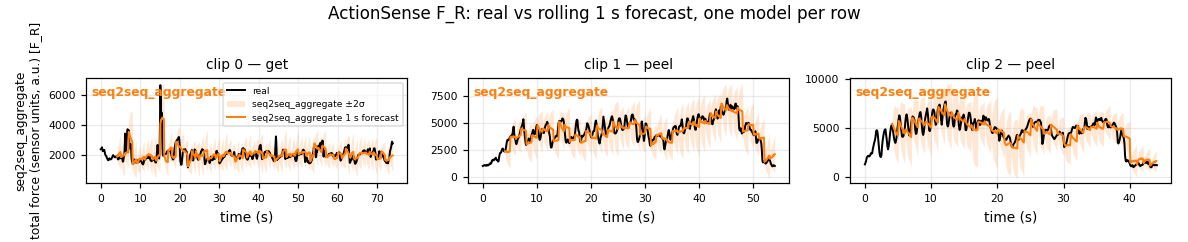
\includegraphics[width=\textwidth]{docs/actionsense/results/corpus-aggregate/as_preds_seq2seq_corpus_F_R.png}%
    }{\placeholderfigure{0.86in}{Upload the ActionSense Seq2Seq full-corpus $F_R$ forecast plot.}}
    \IfFileExists{docs/actionsense/results/corpus-aggregate/as_preds_probgru_corpus_F_R.png}{%
        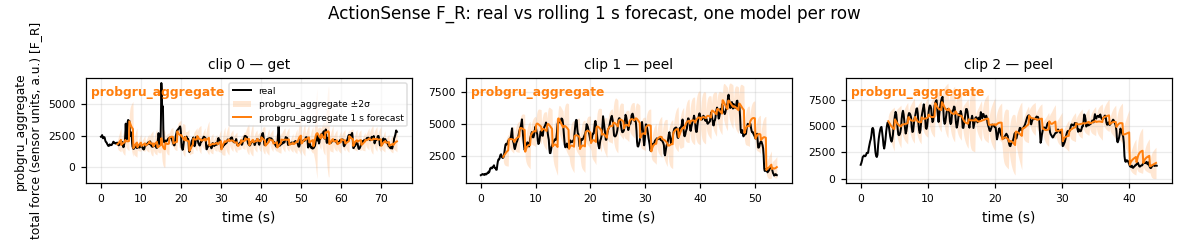
\includegraphics[width=\textwidth]{docs/actionsense/results/corpus-aggregate/as_preds_probgru_corpus_F_R.png}%
    }{\placeholderfigure{0.86in}{Upload the ActionSense ProbGRU full-corpus $F_R$ forecast plot.}}
    \caption{Representative held-out ActionSense right-hand force forecasts with 3~s histories and a 1~s horizon. Black denotes the measured signal, orange the forecast mean, and shading $\pm2$ predicted standard deviations. The three recordings are illustrative; quantitative comparisons use all 290 recordings.}
    \label{fig:pointwise_trajectory}
\end{figure*}

\subsection{Physical Representation}
\label{sec:results_representation}

Within each OpenTouch backbone, physical-state input has the highest skill and lowest Hausdorff ratio on every target (Table~\ref{tab:opentouch_results}). CNN consistently beats flatten under Seq2Seq, but not under ProbGRU, where flatten is better for $c^y$ on both axes. Thus convolutional advantage over flatten does not imply that raw maps outperform the physical representation.

Only 100 of 299 ActionSense recordings contain raw maps, so no map arm shares the full-corpus population; frozen map results use different folds and estimators. H3 is therefore supported by OpenTouch, not replicated on full ActionSense. \emph{Physical representation} denotes compact force and CoP; ``spatial moment'' denotes only its computation.

\subsection{Action-Level Predictability}
\label{sec:results_actions}

Actions are H4's primary unit. For 3~s Seq2Seq, \emph{slice} has the highest $\Rtwo$ (.736), \emph{open} the lowest (.259), and \emph{open/close} the lowest Hausdorff distance (2.283). Action $\Rtwo$ rankings are stable across runs ($\rho=.868$--$.996$) and track persistence $\Rtwo$ ($\rho=.969$), but not Hausdorff distance ($\rho=.051$--$.116$).

Seq2Seq has lower Hausdorff distance on 13 of 14 actions, but the gap concentrates in \emph{clean} ($n=55$): Seq2Seq versus ProbGRU gives $\Rtwo=.634/.469$, skill $.110/-.934$, and Hausdorff ratio $.809/1.033$. Because \emph{clean} is smooth, abruptness alone cannot explain the outlier. These point estimates support action heterogeneity, but without a grouped bootstrap the formal smooth--abrupt H4 remains unresolved.

% Generated directly from the two 3 s shared-scorer CSVs by
% scripts/actionsense/plot_corpus_action_predictability.py.
\begin{figure*}[t]
    \centering
    \IfFileExists{docs/actionsense/results/corpus-aggregate/action_predictability.png}{%
        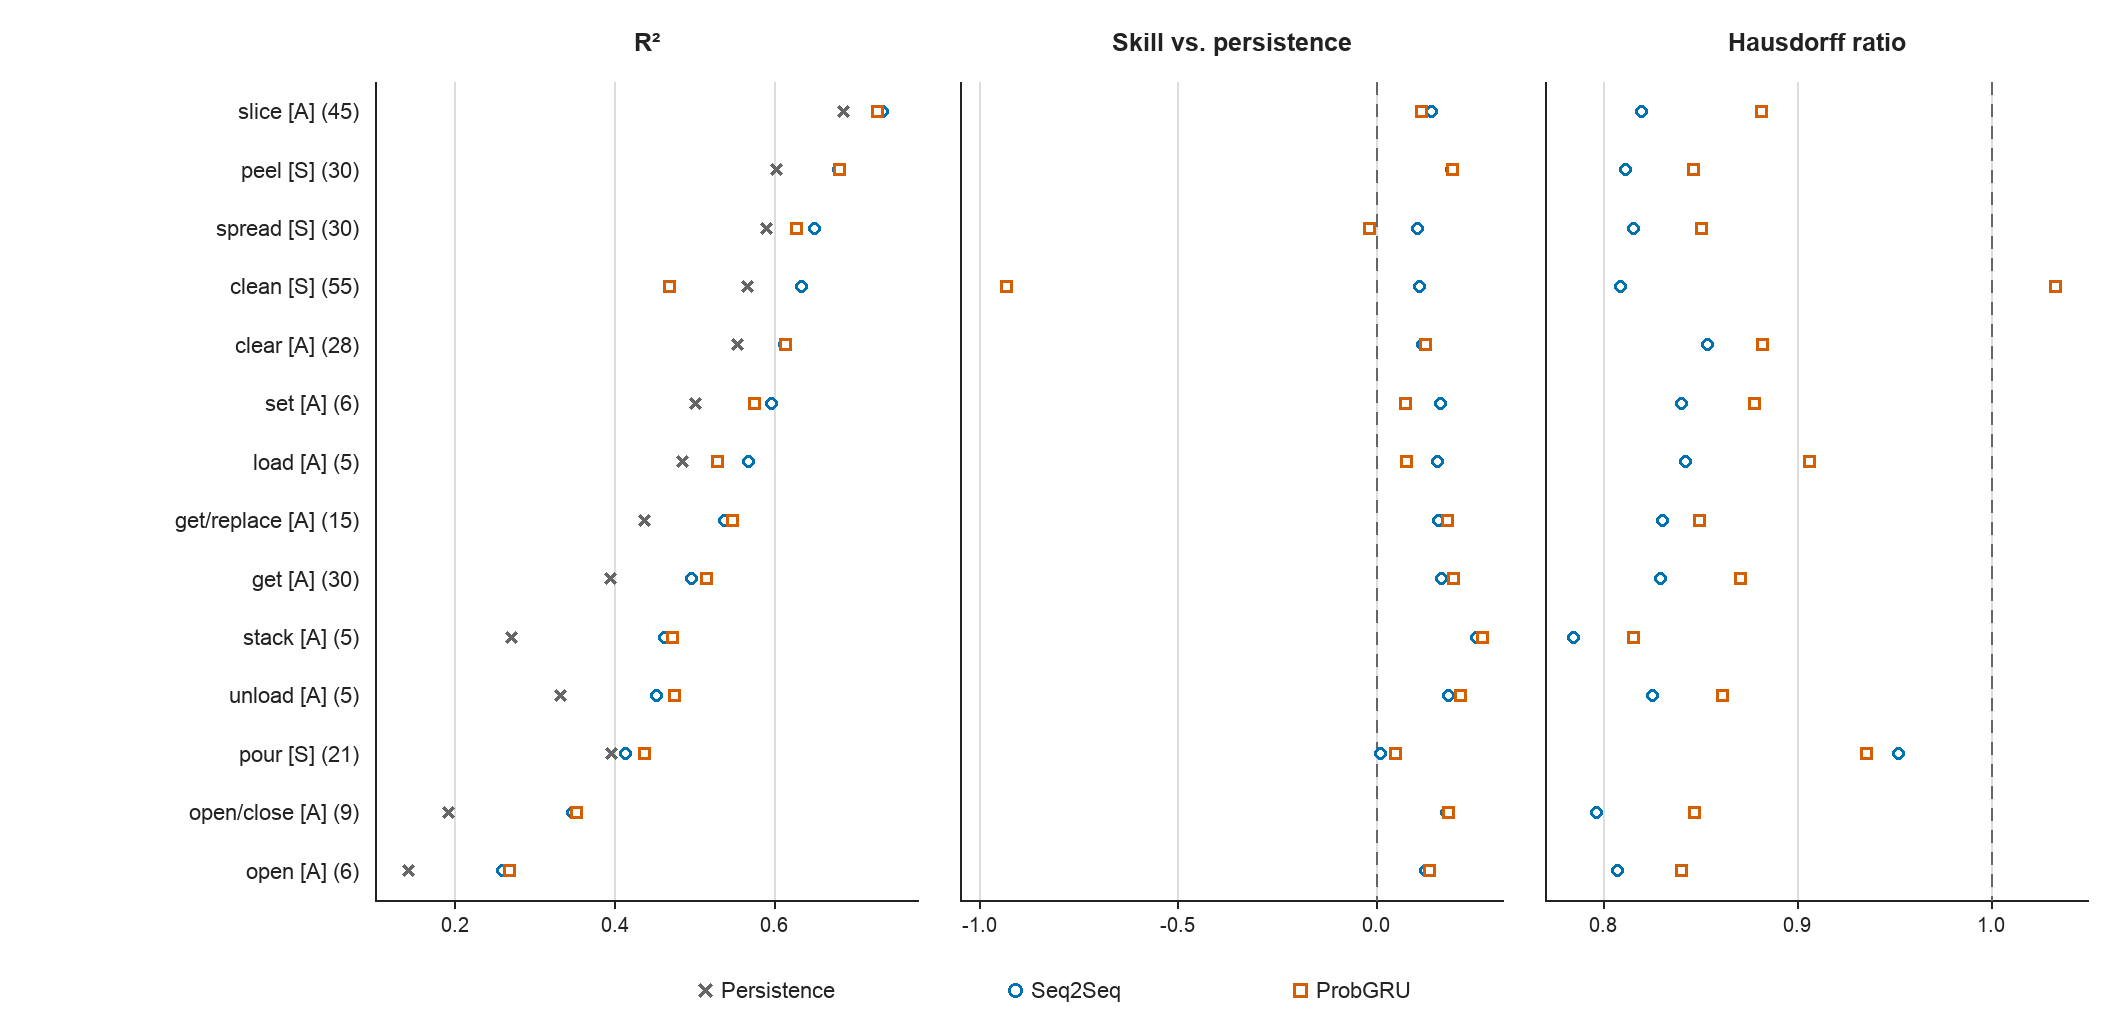
\includegraphics[width=\textwidth]{docs/actionsense/results/corpus-aggregate/action_predictability.png}%
    }{\placeholderfigure{1.22in}{Upload the generated ActionSense full-corpus action-predictability plot.}}
    \caption{ActionSense 3~s per-action point estimates, sorted by Seq2Seq $\Rtwo$. Brackets mark the prespecified abrupt [A] and smooth [S] labels; parentheses give scored recordings. Dashed lines are persistence references. No inferential intervals are available for these full-corpus action contrasts.}
    \label{fig:action_predictability}
\end{figure*}

\paragraph{Predictability synthesis.}
The results separate persistence, pointwise gain, and trajectory geometry. OpenTouch AR matches learned models pointwise, while seasonal naive leads only in shape. ActionSense Seq2Seq improves both axes; ProbGRU improves shape despite negative skill, chiefly because of one action. Physical-state inputs lead on OpenTouch, and ActionSense varies by action. Pointwise accuracy alone therefore cannot establish trajectory recovery.

\section{Discussion and Limitations}
\label{sec:discussion}
\label{sec:limitations}

Smooth tactile trajectories change less over the horizon, directly reducing persistence error. That is a statement about the observed process. Once persistence is already strong, however, a learned model has less additional structure to capture. Conversely, abrupt signals weaken persistence but often contain event timing that is unavailable in tactile history alone. This causal decomposition explains why temporal signal properties track intrinsic predictability while the coarse semantic class has no reliable $\dRtwo$.

For an anticipatory controller, a forecast that merely tracks local load can still provide a slowly varying state estimate, but it should not be interpreted as foreknowledge of contact onset, loss, or slip. Those events may require the commanded action, proprioception, or exteroceptive context. The present results recommend three reporting rules for tactile forecasting: (i) state baseline correction and report $\Rdiff$ beside skill; (ii) weight recordings or interaction episodes rather than frames; and (iii) pair pointwise error with a trajectory-shape diagnostic. These rules make it harder for sensor pedestal, clip duration, or amplitude attenuation to masquerade as improved dynamics.

The long-horizon gap suggests modeling a slow contact envelope separately from fast residuals. Yet fast residual timing may be conditionally predictable only from future action or object motion. A decisive next experiment is therefore not simply a larger recurrent network; it is a controlled comparison of tactile-only history against causally available action, pose, and vision, followed by a downstream contact-loss or slip-warning evaluation.

The formal smooth/abrupt test is limited to OpenTouch and is imbalanced (299 versus 2,544 clips). Semantic labels are a coarse proxy for measured signal smoothness and include context-dependent verbs. Neither corpus provides participant identifiers adequate for a participant-disjoint claim: ActionSense is held out by recording and OpenTouch by location. Force remains in sensor-specific arbitrary units. ActionSense target construction uses a complete-recording percentile, while OpenTouch target correction and map calibration pool frames within acquisition shards; these offline sensor corrections are not restricted to the forecasting history or refit within each training fold. ActionSense representation comparisons remain limited to the frame-pooled, unmasked frozen neural sweep; the full-corpus scorer is recording-balanced but also omits the low-force CoP mask. The Gaussian error model is misspecified for heavy-tailed residuals. Finally, this study measures forecasts offline and contains no robot or closed-loop control experiment; its robotics implications should therefore be read as testable design guidance rather than demonstrated control benefit.

\section{Conclusion}
\label{sec:conclusion}

One-second tactile predictability is jointly determined by contact dynamics and evaluation design. Smooth signals strengthen persistence, but the smooth/abrupt action class does not reliably identify where learned models add predictive value. Across sensor geometries and model families, positive pointwise scores primarily reflect local-level recovery, while rapid contact dynamics remain poorly anticipated. Reporting intrinsic persistence difficulty, clip-balanced $\Rtwo$, and trajectory shape together turns this apparent contradiction into a consistent result and clarifies which forecasting gains would matter for future robotic control.

% Omit acknowledgments during anonymous review if they reveal identity.

\begin{thebibliography}{00}

\bibitem{kappassov2015tactile}
Z. Kappassov, J.-A. Corrales, and V. Perdereau, ``Tactile sensing in dexterous robot hands---Review,'' \emph{Robot. Auton. Syst.}, vol. 74, pp. 195--220, 2015, doi: 10.1016/j.robot.2015.07.015.

\bibitem{sundaram2019glove}
S. Sundaram, P. Kellnhofer, Y. Li, \emph{et al.}, ``Learning the signatures of the human grasp using a scalable tactile glove,'' \emph{Nature}, vol. 569, no. 7758, pp. 698--702, 2019, doi: 10.1038/s41586-019-1234-z.

\bibitem{veiga2015stabilizing}
F. F. Veiga, H. van Hoof, J. Peters, and T. Hermans, ``Stabilizing novel objects by learning to predict tactile slip,'' in \emph{Proc. IEEE/RSJ Int. Conf. Intell. Robots Syst. (IROS)}, 2015, pp. 5065--5072, doi: 10.1109/IROS.2015.7354090.

\bibitem{tian2019manipulation}
S. Tian, F. Ebert, D. Jayaraman, \emph{et al.}, ``Manipulation by feel: Touch-based control with deep predictive models,'' in \emph{Proc. IEEE Int. Conf. Robot. Autom. (ICRA)}, 2019, pp. 818--824, doi: 10.1109/ICRA.2019.8794219.

\bibitem{zhang2021dynamic}
Q. Zhang, Y. Li, Y. Luo, \emph{et al.}, ``Dynamic modeling of hand--object interactions via tactile sensing,'' in \emph{Proc. IEEE/RSJ Int. Conf. Intell. Robots Syst. (IROS)}, 2021, pp. 2874--2881, doi: 10.1109/IROS51168.2021.9636361.

\bibitem{mandil2022actp}
W. Mandil, K. Nazari, and A. Ghalamzan, ``Action conditioned tactile prediction: Case study on slip prediction,'' in \emph{Robotics: Science and Systems XVIII}, 2022, doi: 10.15607/RSS.2022.XVIII.070.

\bibitem{nunes2020benchmarking}
M. S. Nunes, A. Dehban, P. Moreno, and J. Santos-Victor, ``Action-conditioned benchmarking of robotic video prediction models: A comparative study,'' in \emph{Proc. IEEE Int. Conf. Robot. Autom. (ICRA)}, 2020, pp. 8316--8322, doi: 10.1109/ICRA40945.2020.9196839.

\bibitem{delpreto2022actionsense}
J. DelPreto, C. Liu, Y. Luo, \emph{et al.}, ``ActionSense: A multimodal dataset and recording framework for human activities using wearable sensors in a kitchen environment,'' in \emph{Advances in Neural Information Processing Systems}, vol. 35, pp. 13800--13813, 2022, doi: 10.52202/068431-1003.

\bibitem{song2025opentouch}
Y. R. Song, J. Li, R. Fu, \emph{et al.}, ``OpenTouch: Bringing full-hand touch to real-world interaction,'' arXiv:2512.16842, 2025.

\bibitem{gao2022simvp}
Z. Gao, C. Tan, L. Wu, and S. Z. Li, ``SimVP: Simpler yet better video prediction,'' in \emph{Proc. IEEE/CVF Conf. Comput. Vis. Pattern Recognit. (CVPR)}, 2022.

\bibitem{hyndman2006accuracy}
R. J. Hyndman and A. B. Koehler, ``Another look at measures of forecast accuracy,'' \emph{Int. J. Forecasting}, vol. 22, no. 4, pp. 679--688, 2006.

\bibitem{salinas2020deepar}
D. Salinas, V. Flunkert, J. Gasthaus, and T. Januschowski, ``DeepAR: Probabilistic forecasting with autoregressive recurrent networks,'' \emph{Int. J. Forecasting}, vol. 36, no. 3, pp. 1181--1191, 2020, doi: 10.1016/j.ijforecast.2019.07.001.

\bibitem{dubuisson1994modified}
M.-P. Dubuisson and A. K. Jain, ``A modified Hausdorff distance for object matching,'' in \emph{Proc. Int. Conf. Pattern Recognit.}, 1994, pp. 566--568.

\end{thebibliography}

\end{document}
